% xetex compatible variant that support TTF fonts according to company rules
\documentclass[ignorenonframetext, professionalfonts, hyperref={unicode}]{beamer}

\usetheme{Epam}

\usepackage{fontspec}
\setsansfont{SourceSansPro-Regular}
%\setbeamerfont{frametitle}{family=\fontspec{Oswald}}
\setbeamerfont{frametitle}{family=\fontspec{Oswald}}
\setbeamerfont{block title}{family=\fontspec{Oswald}}

%\setmainfont{Times New Roman}
\defaultfontfeatures{Mapping=tex-text}
\defaultfontfeatures{Ligatures=TeX}

%\setsansfont{Arial}
%\setromanfont{Trebuchet MS}

\usepackage{cmap}
\usepackage{graphicx}

\usepackage{textcomp}

\usepackage{beamerthemesplit}

\usepackage{ulem}

\usepackage{verbatim}
\usepackage{import}

\usepackage{listings}
\lstloadlanguages{bash}

\lstset{escapechar=`,
	captionpos=b,
	extendedchars=false,
	language=sh,
%	frame=single,
	tabsize=2, 
	columns=fullflexible, 
%	basicstyle=\scriptsize,
	keywordstyle=\color{blue}, 
	commentstyle=\itshape\color{brown},
%	identifierstyle=\ttfamily, 
	stringstyle=\mdseries\color{green}, 
	showstringspaces=false, 
	numbers=left, 
	numberstyle=\footnotesize, 
	breaklines=true, 
	inputencoding=utf8,
	keepspaces=true,
	morekeywords={u\_short, u\_char, u\_long, in\_addr}
	}

\definecolor{darkgreen}{cmyk}{0.7, 0, 1, 0.5}

\lstdefinelanguage{diff}
{
    morekeywords={+, -},
    sensitive=false,
    morecomment=[l]{//},
    morecomment=[s]{/*}{*/},
    morecomment=[l][\color{darkgreen}]{+},
    morecomment=[l][\color{red}]{-},
    morestring=[b]",
}

\author[Epam]{{\bf Epam}\\Low Level Programming Department}

%\institution[EPAM]{EPAM}
%\logo{\includegraphics[width=1cm]{logo.png}}

\graphicspath{{../../slides/cmdline/clipart/}{../../slides/bash/clipart/}}

\bibliographystyle{unsrt}
\setbeamertemplate{bibliography item}{\insertbiblabel}

\AtBeginSection[]{%
  \begin{frame}<beamer>
    \frametitle{}
    \tableofcontents[
        sectionstyle=show/shaded, hideallsubsections ]
  \end{frame}
  \addtocounter{framenumber}{-1}% If you don't want them to affect the slide number
}

% \regex for regular expressions
\newcommand{\regex}[1]{ %
\expandafter{$\ulcorner{\color{blue}\texttt{#1}}\lrcorner$} %
}



\title{Введение в GNU/Linux}


%%%%%%%%%%%%%%%%%%%%%%%%%%%%%%%%%%%%%%%%%%%%%%%%%
%%%%%%%%%% Begin Document  %%%%%%%%%%%%%%%%%%%%%%
%%%%%%%%%%%%%%%%%%%%%%%%%%%%%%%%%%%%%%%%%%%%%%%%%

\begin{document}

\begin{frame}
	\frametitle{}
	\titlepage
	\vspace{-0.5cm}
	\begin{center}
	%\frontpagelogo
	\end{center}
\end{frame}


%%%%%%%%%%%%%%%%%%%%%%%%%%%%%%%%%%%%%%%%%   
%%%%%%%%%% Content starts here %%%%%%%%%%
%%%%%%%%%%%%%%%%%%%%%%%%%%%%%%%%%%%%%%%%%

\section{Multiuser UNIX}
\subsection{File permissions}
%\mode<all>{\import{../../slides/cmdline/}{access_rights.tex}}
\mode<all>{\begin{frame}[fragile]{User identifier}

\begin{block}{User ID (UID)}
\alert{A user ID (UID)} is a unique positive integer assigned by a Unix-like operating system to each user.
\end{block}

Commands to determine who you are
  \begin{itemize}
    \item \verb|id|
    \item \verb|whoami|
    \item \verb|loginctl list-users|
    \item \verb|loginctl show-user val|
    \item \verb|who|, \verb|w|
  \end{itemize}
Users configuration file:  \alert{/etc/password}
\end{frame}
}
\mode<all>{\begin{frame}[fragile]{Group identifier}

\begin{block}{Group ID (GID)}
\alert{A group identifier} is a numeric value used to represent a specific group.
Groups are collections of zero or more users.
\end{block}

\begin{block}{Default group}
 Every user must be a member of at least one group, the \alert{primary group} which is identified by the numeric GID
\end{block}

Commands to determine group
  \begin{itemize}
    \item \verb|id, id username|
    \item \verb|groups, groups username|
  \end{itemize}
Group configuration file:  \alert{/etc/group}
\end{frame}
}
\mode<all>{\begin{frame}[fragile]{Владельцы файлов.Определения}

  В UNIX (и Linux) любой файл имеет двух владельцев:
  \begin{enumerate}
    \item владельца-пользователя
    \item владельца-группу.
  \end{enumerate} 
  \lstinputlisting{../../slides/cmdline/samples/ls-l} 
  \pause

  \begin{itemize}
    \item \alert{Группой} - определенный список пользователей системы.
    \item Пользователь может быть членом нескольких групп. 
    \item Одна группа пользователя является первичной\footnote{primary (eng.)}, а остальные - дополнительными.
  \end{itemize}
  \small{Замечание: владелец-пользователь не обязан входить в группу-владельца.}
  \lstinputlisting{../../slides/cmdline/samples/id} 

\end{frame}
}
\mode<all>{\begin{frame}[fragile]{Владельцы файла. Внутреннее представление}
  \begin{itemize}
    \item \alert{Владелец-пользователь} и \alert{владелец-группа} файла определяются по идентификаторам \alert{UID}\footnote{UID - User IDentifier} и \alert{GID}\footnote{GID - Group IDentifier}, а не по именам. 
\lstinputlisting{../../slides/cmdline/samples/ls-nl} \pause
    \item Зарегистрированные пользователи и группы определены в файлах \alert{/etc/passwd} и \alert{/etc/group} \newline
    Следствие: могут существовать файлы, принадлежащие не зарегистрированным в системе пользователям и группам. \pause
    \item Новые файлы создаются с владельцем-пользователем, запустившим команду создания и его первичной группой, как владельцем группой. \pause
  \end{itemize}

\end{frame}
}
\mode<all>{\begin{frame}[fragile]{Управление владельцами}

  Команды изменения владельцев
  \begin{itemize} 
    \item \alert{chown} : смена владельца-пользователя \newline
      Пример: \verb+chown sys something.doc+
    \item \alert{chgrp} : смена владельца-группы \newline
      Пример: \verb+chgrp adm file.txt+
  \end{itemize} \pause

  Кто может сменить владельцев?
  \begin{itemize}
    \item группу - владелец-пользователь для группы, к которой он сам принадлежит
    \item администратор (root, UID=0)\footnote{На пользователя c UID=0 не распространяются ограничения прав доступа} 
  \end{itemize} 
\end{frame}
}
\mode<all>{\begin{frame}[fragile]{root user}
 Special user with all rights. Use cases:
  \begin{itemize} 
    \item Edit system configuration file;
    \item Add and remove users;
    \item Change file permissions;
    \item Stop and start any processes.
  \end{itemize}
How to get root access? 
 \break
  login as root. Use command: su, sudo. Start application with SUID bit 
\end{frame}
}
\mode<all>{\begin{frame}[fragile]{Users management}
    \begin{columns}
        \column{0.5\textwidth}
        \begin{itemize} 
          \item useradd
          \item usermod
          \item userdel
          \item passwd
        \end{itemize}

        \column{0.5\textwidth}
        \begin{itemize} 
          \item groupadd
          \item groupmod
          \item groupdel
        \end{itemize}
    \end{columns}
\end{frame}
}
\mode<all>{\begin{frame}{Введение в права доступа}
  У каждого файла присвоены атрибуты, называемые \alert{правами доступа}.
  
  Проверяются при каждом обращении к любому файлу с любой операцией чтение, запись, выполнение (\alert{r}ead, \alert{w}rite, e\alert{x}ecute)

\end{frame}
}
\mode<all>{\begin{frame}{Классы доступа и права доступа}
  В UNIX три базовых типа (класса) доступа:
  \begin{enumerate}
    \item \alert{u} (user) для владельца-пользователя
    \item \alert{g} (group) для владельца-группы         
    \item \alert{o} (other) для всех остальных \pause
  \end{enumerate}

  \begin{tabular}{c | c | c | c}
     & u & g & o \\ \hline
   read & 1 & 1 & 0 \\ \hline
   write & 1 & 1 & 0 \\ \hline
   execute & 0 & 0 & 0 \\ 
  \end{tabular}
\end{frame}
}
\mode<all>{\begin{frame}[fragile]{Разбор прав доступа в выводе ls -l}

  Вывод команды \alert{ls -l} содержит информацию о правах доступа:

  \lstinputlisting[basicstyle=\small,breaklines=false]{samples/ls-l-details}

  Позиции:
  \begin{itemize}
    \item 0 - тип  файла: - обычный;
    \item 1-3 - (\alert{u}) права доступа для владельца-пользователя.
    \item 4-6 - (\alert{g}) права доступа для владельца-группы.
    \item 7-9 - (\alert{o}) права доступа для остальных.
  \end{itemize}
\end{frame}
}
\mode<all>{\begin{frame}{Значение прав доступа. Файлы и ссылки}

  \begin{block}{Обычные файлы}
    \begin{itemize}
      \item чтение \alert{(r)} надо, чтобы прочитать файл
	\footnote{Для успешного запуска скрипта необходимо установить атрибут \alert{r}, чтобы командный интерпретатор мог построчно считывать текст скрипта.}
      \item запись \alert{(w)}, чтобы файл изменить
      \item выполнение \alert{(x)}, чтобы запустить программу или скрипт.
    \end{itemize}
  \end{block} \pause

  \begin{block}{Символические ссылки}
    \small{Права символических ссылок совпадают с файлом, на который она указывает. На самой ссылке стоит 'всем всё разрешено'.}
  \end{block}

\end{frame}
}
\mode<all>{\begin{frame}{Значение прав доступа. Каталоги}
  \begin{block}{Каталоги}
    \begin{itemize}
      \item \alert{(r)} позволяет получить имена (и только имена) файлов в нём\footnote{ls dir}. 
      \item \alert{(w)} позволяет изменять имена файлов. Например удалить файл или переименовать файл \footnote{rm dir/file} 
      \item \alert{(x)} позволяет "выполнить" каталог\newline
	то есть заглянуть в метаданные  и получить полную информацию о каталоге и файлах в нём\footnote{ls -l dir}.
    \end{itemize}
  \end{block}
\end{frame}
}
\mode<all>{\begin{frame}[fragile]{chmod: change access mode}
    \begin{itemize}
      \item \verb;chmod 400 file ; установить права в цифровой форме
      \item \verb;chmod u=rw file;  установить права
      \item \verb;chmod ugo+rw file; добавить права
      \item \verb;chmod ug-rw file; удалить права
    \end{itemize}
\end{frame}
}
\mode<all>{\begin{frame}[fragile]{Special modes}

\begin{block}{SUID (set user ID), SGID (set group ID) }
Установка битов SUID или SGID позволит пользователям запускать исполняемые файлы от имени владельца (или группы) запускаемого файла
\end{block}
\verb|chmod 4755 plu.txt| или \verb|chmod u+s plu.txt|

\begin{block}{Sticky bit mode}
Каталог с установленным sticky-битом означает, что удалить файл из этого каталога может только владелец файла 
\end{block}
\verb|chmod 1755 plu| или \verb|chmod +t plu|

\end{frame}
}
\mode<all>{\begin{frame}[fragile]{Default access mode: umask}

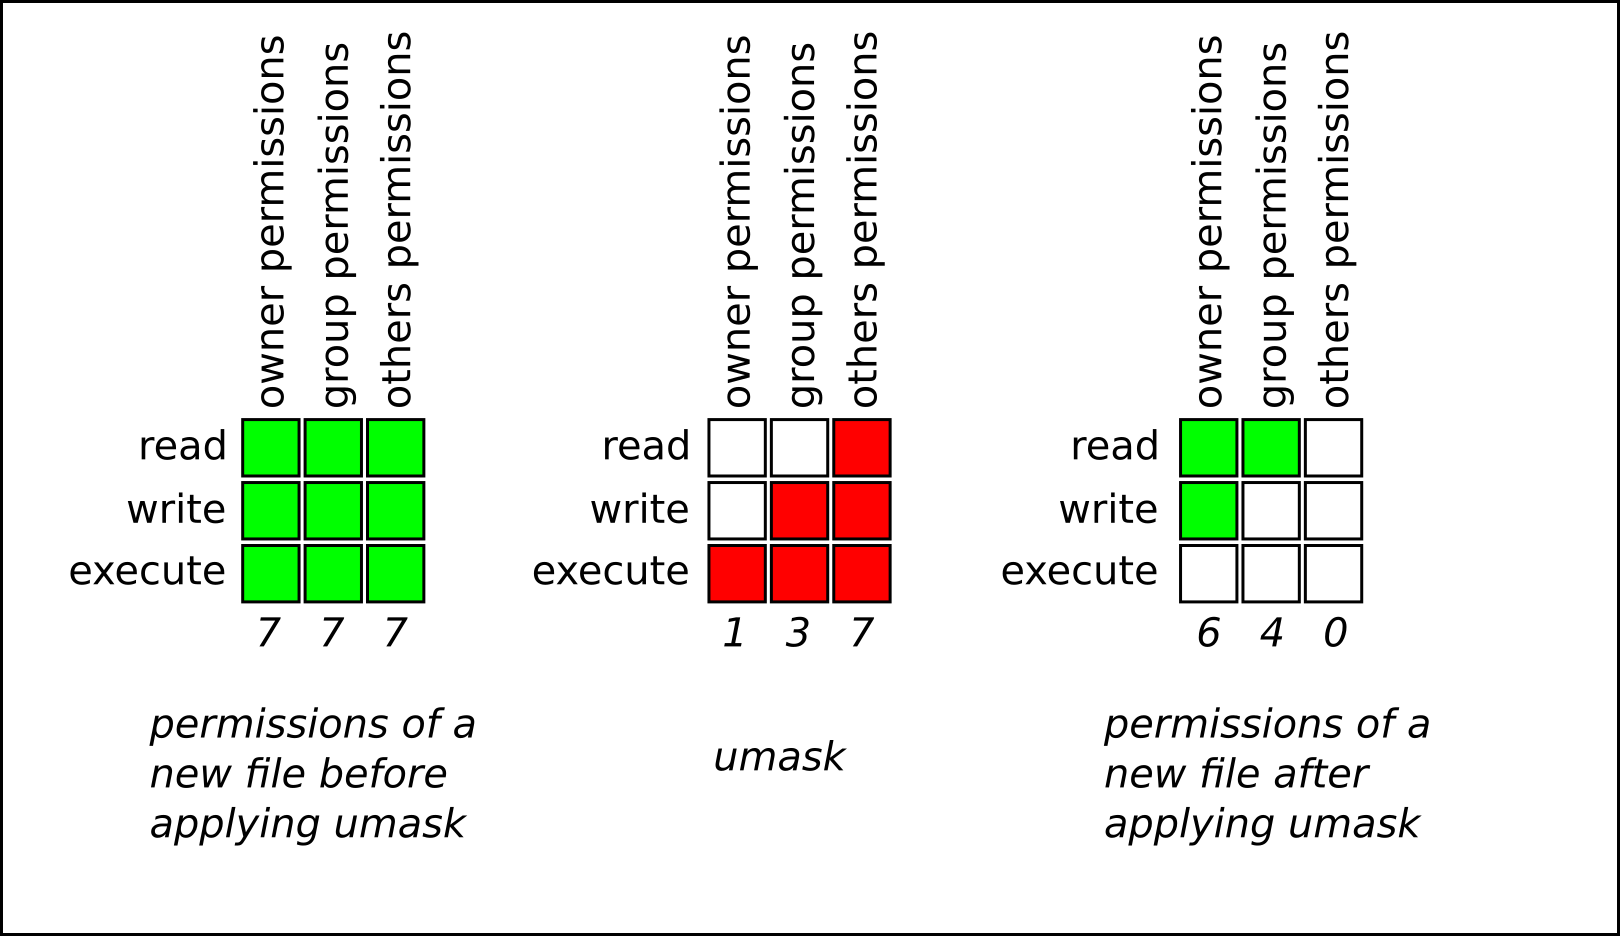
\includegraphics[width=0.9\textwidth]{../../slides/cmdline/clipart/Users_Groups-Umask_Example.png}

\end{frame}
}
\section{Processes management}
\mode<all>{\import{../../slides/cmdline/}{processes.tex}}
%\mode<all>{\begin{frame}{Процессы. Общая информация}
\begin{columns}
        \column{0.8\textwidth}
  \begin{block}{Процесс}
    \begin{itemize}
      \item Данные с диска загружаются в оперативную память.
      \item Процесс состоит из инструкций, выполняемых процессором, данных и информации о выполняемой задаче 
      \item Программа запускает 1 или более процессов. 
    \end{itemize} 
  \end{block}
        \column{0.3\textwidth}
        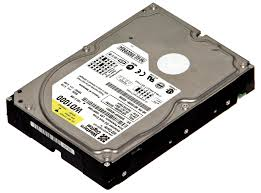
\includegraphics[height=2cm]{hw_hdd.jpg} \break
        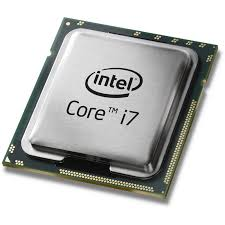
\includegraphics[height=2cm]{hw_cpu.jpg} \break
        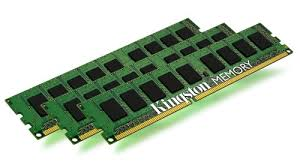
\includegraphics[height=2cm]{hw_memory.jpg} 
\end{columns}
\end{frame}

\begin{frame}{Процессы. Изоляция}
    \begin{itemize}
      \item Процессы изолированы друг от друга\footnote{нет доступа к памяти и стеку, открытым файлам и порядку выполения}.
      \item Для обмена данными используется система межпроцессного взаимодействия (IPC)
      \item Следствие: пользователи могут запускать несколько экземпляров одной и той же программы. 
    \end{itemize}
\end{frame}


}
%\mode<all>{\begin{frame}{Файлы и процессы. Права доступа}

  \begin{block}{Связь с файлами}
    Процессы запускаются из файлов (двоичных программ или скриптов).
  \end{block}

  \begin{block}{Права доступа}
    Процессы работают с правами пользователя, их запустившего\footnote{Если не установлены SUID или SGID биты на файле программы}
  \end{block}

\end{frame}
}
%\mode<all>{\begin{frame}{Виды процессов}
% TODO картинку с демоном
  \begin{block}{Демоны}
    Неинтерактивные процессы, выполняются в фоновом режиме. Не связаны ни с одним пользовательским сеансом и не могут непосредственно управляться пользователем. \newline
    Примеры: \alert{sshd}, \alert{apache}, \alert{cron}, \alert{samba}
  \end{block} \pause

  \begin{block}{Системные процессы}
    Часть ядра и всегда расположены в оперативной памяти. \newline
    Примеры: диспечер подкачки памяти ( \alert{[kswapd0]} )
  \end{block} \pause

  \begin{block}{Прикладные процессы}
    все остальные процессы. Запускаются в рамках пользовательского сеанса. \newline
    Примеры: \alert{ls}, \alert{bash}, \alert{vim}, \alert{find}, \alert{mysql}

  \end{block}

\end{frame}
}
%\mode<all>{\begin{frame}[fragile]{Практика: утилиты просмотр процессов}
    
  \begin{itemize}
      \item \alert{ps} - список запущенных процессов.\newline
	Популярные ключи: \alert{-u username}, 
	\alert{ax}\footnote{ \alert{ax} для BSD, \alert{-e} в SystemV}, 
	\alert{aux}\footnote{ \alert{aux} для BSD, \alert{-ef} в SystemV}
\lstinputlisting{samples/ps-ax}
      \item \alert{top} - интерактивный список процессов
\lstinputlisting{samples/top}
    \end{itemize}

\end{frame}
}
%\mode<all>{\begin{frame}{Состояния процесса}
  % TODO
\end{frame}
}
%\mode<all>{\begin{frame}{Виды межпроцессного взаимодействия (IPC)}

  \begin{block}{Пользовательские IPC}
    \begin{enumerate}
      \item \alert{файлы}
      \item \alert{каналы (трубы)} - именованные (FIFO) и неименованные (в Shell)\pause
      \item \alert{сигналы} - уведомление о возникновении события
    \end{enumerate}
  \end{block}\pause

  \begin{block}{IPC Для программистов}
    \begin{enumerate}
      \item \alert{разделяемая память}
      \item \alert{семафоры}
      \item \alert{очереди сообщений}
    \end{enumerate}
  \end{block}

\end{frame}
}
%\mode<all>{\begin{frame}{Сигналы}
  \begin{block}{Сигнал}
    \begin{enumerate}
      \item Cпособ передачи уведомления о возникновении какого-либо события.
      \item Сигнал может идти от одного процесса другому или от ядра ОС какому-либо процессу.
      \item Номер сигнала - единственная информация, которую он передаёт.
    \end{enumerate}
  \end{block} \pause

  \begin{block}{Права доступа}
    \begin{itemize}
      \item Пользователь может посылать сигналы только тем процессам, владельцем которых он является.
      \item \alert{root} может посылать сигналы любому процессу.
    \end{itemize}
  \end{block}

\end{frame}
}
%\mode<all>{\begin{frame}[fragile]{Работа с сигналами}
  \small Информация о сигналах: \alert{man 7 signal}, \alert{kill -l}
  \begin{block}{Популярные сигналы}
    \tiny
    \begin{tabular}{l|c|c|l}
      Сигнал & Значение & Действие
      .умолч.& Комментарий \\ \hline 
      SIGHUP &    1     &  Term   &  Обрыв соед. терминала или смерть упр. процесса \\
      SIGINT &    2     &  Term   & Прерывание с клавиатуры (Ctrl+C) \\
      SIGKILL &   9     &  Term   & Убить процесс \\
      SIGSEGV &   11    &  Core   & Segmentation fault \\
      SIGPIPE &   13    &  Term   & Broken pipe: запись в канал без читателей\\
      SIGTERM &   15    &  Term   & Прекратить процесс \\
      SIGCONT &   18    &  Cont   & Продолжить выполнение \\
      SIGSTOP &   19    &  Stop   & Остановить 
    \end{tabular}
  \end{block} \pause

  \begin{block}{Утилиты управления}
    \begin{itemize}
      \item \alert{kill} - послать сигнал процессу (по PID)
      \item \alert{killall} - послать сигнал процессам по имени
    \end{itemize}
  \end{block}

\end{frame}
}
\subsection{OS initialization system.}
\mode<all>{\begin{frame}{init}
	Менеджер управления работой системой и сервисами.
	
	\bigskip

	\center{\large PID = 1}

	\bigskip

	\begin{block}{Наиболее известные}
		\begin{itemize}
			\item SysVInit
			\item systemd
			\item upstart
		\end{itemize}
	\end{block}
\end{frame}

\begin{frame}{SysVInit}
	\begin{block}{Управление}
		\begin{itemize}
			\item kernel boot parameters: <N> -- runlevel
			\item утилита {\tt runlevel}
			\item утилита {\tt init}
		\end{itemize}
	\end{block}

	\scriptsize
	\begin{block}{Runlevel}
		\begin{table}
			\begin{tabular}{| c | l | }
			\hline
			Runlevel & Описание\\
			\hline
			0	& Выключить систему \\
			1,s,single & Однопользовательский режим \\
			2	& Многопользовательский режим без графики. Без сетевых сервисов.\\
			3	& Многопользовательский режим без графики. Полноценная сеть. \\
			4	& Определяется на хосте\\
			5	& Многопользовательский режим с графикой.\\
			6	& Перезагрузка\\
			emergency & Аварийная оболочка \\
			\hline
			\end{tabular}
		\end{table}
	\end{block}
\end{frame}

\begin{frame}{SysVInit: сервисы}
	\begin{block}{Управление}
		\begin{itemize}
			\item утилита {\tt service}
			\item утилита {\tt chkconfig}
		\end{itemize}
	\end{block}

	\begin{block}{Сервисы}
		\begin{itemize}
			\item {\tt /etc/rc.d/init.d}
			\item {\tt /etc/rc.d/rc.N}\footnote{N=runlevel}
		\end{itemize}
	\end{block}
\end{frame}

\begin{frame}{systemd}
	\begin{block}{Управление}
		\begin{itemize}
			\item kernel boot parameters\\
				{\tt systemd.unit=rescue.target} \\
			\item утилита {\tt systemctl} \\
				{\tt systemctl isolate multi-user.target} \\
				{\tt systemctl set-default single.target}
		\end{itemize}
	\end{block}

	\begin{block}{targets}
		\tiny
		\begin{table}
			\begin{tabular}{| c | l | l | }
			\hline
			Runlevel & Описание\\
			\hline
			0	& poweroff.target & Выключить систему \\
			1,s,single & rescue.target  & Однопользовательский режим \\
			2	& multi-user.target & Многопользовательский режим без графики. Без сетевых сервисов.\\
			3	& multi-user.target & Многопользовательский режим без графики. Полноценная сеть. \\
			4	& multi-user.target & Определяется на хосте\\
			5	& graphical.target & Многопользовательский режим с графикой.\\
			6	& reboot.target & Перезагрузка\\
			emergency & emergency.target & Аварийная оболочка \\
			\hline
			\end{tabular}
		\end{table}
	\end{block}
\end{frame}

\begin{frame}{systemd: сервисы}
	\begin{block}{Управление}
		\begin{itemize}
			\item утилита {\tt systemctl}
		\end{itemize}
	\end{block}

	\begin{block}{Сервисы}
		\begin{itemize}
			\item {\tt /lib/systemd/system/}
			\item {\tt /etc/systemd/system/}
		\end{itemize}
	\end{block}
\end{frame}
}

%\section{User management}
%\mode<all>{\input{../../slides/multiuser/account_files.tex}}
%\mode<all>{\input{../../slides/multiuser/pam.tex}}


\section{Configure network settings}
\mode<all>{\begin{frame}{Сетевая подсистема Linux}

	\begin{block}{Cетевой интерфейс}

		Сетевой интерфейс в Linux -– это абстрактный \alert{именованный} объект,  используемый для передачи 
		данных через некоторую линию связи без привязки к ее (линии связи) реализации.
	\end{block}
\end{frame}

\begin{frame}{Сетевая подсистема Linux}

	\center\includegraphics[width=0.9\textwidth]{../../slides/networking/06-netstack.png}

\end{frame}


} % add real config

\subsection{Управление интерфейсами}
\mode<all>{\input{../../slides/networking/interface-management}}

\subsection{Полезные программы}
\mode<all>{\begin{frame}{Полезные утилиты}
	\begin{center}
		\begin{itemize}
			\item netstat / ss
			\item nslookup / dig
			\item ping
			\item traceroute
			\item tcpdump
			\item telnet
			\item netcat
			\item nmap
		\end{itemize}
	\end{center}

\end{frame}


%\begin{frame}{Полезные утилиты: практика}
%
%	\begin{columns}
%		\column{0.5\textwidth}
%		\begin{block}{netstat}
%
%			Узнать:
%			\begin{itemize}
%				\item список используемых сокетов
%				\item серверных сокетов
%				\item имена/pid серверов
%				\item узнать номера портов
%			\end{itemize}
%		\end{block}
%	
%		\pause
%		\column{0.5\textwidth}
%		\begin{block}{telnet/netcat}
%
%			\begin{itemize}
%				\item Чат по протоколу TCP с соседом
%				\item Чат по протоколу UDP с соседом
%				\item Передать текстовый и бинарный файлы
%			\end{itemize}
%	
%			При создании чата использовать {\tt netstat} и {\tt tcpdump}
%			для получения информации о соединении.
%		\end{block}
%	
%	\end{columns}
%\end{frame}
%
%nmap
%1. сканирование соседа
%2. сканирование выделенных портов у соседа (поиск сервера чата) 
%3. узнать список открытых портов на всех машинах в 505
%4. узнать список  работающих машин
%
%tcpdump
%0. pcap файлы/libpcap
%1. запуск монитора
%2. запуск чата
%3. монитор-фильтр-анализ
%
}

\subsection{Маршрутизация}
\mode<all>{\input{../../slides/networking/routing}}
\subsection{iptables}
\mode<all>{\input{../../slides/networking/iptables}}

\end{document}
